%! TEX root = main.tex

\chapter{Sound Propagation}

This chapter analyzes how sound waves propagate in the environment. It isn't concerned with the generation mechanism, but only with propagation in the surrounding medium. Sound can be described as a perturbation of the air pressure field with frequency content in the range \SIrange{20}{20000}{\hertz}.

\section{Equation of Air Motion and Plane Waves}

Considering one-dimensional propagation along the \( x \) axis, the pressure perturbation \( p(x,t) \) satisfies
\[
\frac{\partial^{2} p}{\partial t^{2}} = c^{2} \frac{\partial^{2} p}{\partial x^{2}}
\]
where \( c \) is the sound speed. Under small-signal adiabatic conditions, the sound speed in air can be expressed as
\[
c = \sqrt{\frac{\gamma p_{a}}{\rho}}
\]
where \( \gamma \) is the ratio of specific heats, \( p_{a} \) is the ambient pressure, and \( \rho \) is the air density. A commonly used approximation highlights the dependence of \( c \) on temperature
\[
c = 331.3 + 0.606 \Delta T~\si{\metre\per\second}
\]
where \( \Delta T \) is the temperature in Celsius degrees. A general solution can be written as the superposition of two counter-propagating plane waves
\[
p(x,t) = A e^{-j k x} e^{j \omega t} + B e^{j k x} e^{j \omega t}
\]
where \( A \) and \( B \) are complex amplitudes and the wavenumber is \( k = \omega / c \). The particle velocity \( u(x,t) \) is the speed of air particles subject to the pressure perturbation \( p \). In free field, for a single progressive plane wave traveling in \( +x \) (i.e. \( B = 0 \)), where boundaries are absent, pressure and particle velocity are related by
\[
p = \rho c u
\]
This motivates the definition of wave impedance (also known as acoustic impedance)
\[
z = \frac{p}{u}
\]
For a plane wave, \( z = \rho c \), therefore its value does not depend on the measurement point.

\section{Spherical Waves}

When propagation occurs in three dimensions, the acoustic pressure \( p(x,t) \) satisfies the wave equation
\[
\frac{\partial^{2} p}{\partial t^{2}} = c^{2} \nabla^{2} p
\]
where \( \nabla^{2} \) is the Laplace operator. In Cartesian coordinates,
\[
\nabla^{2} p = \frac{\partial^{2} p}{\partial x^{2}} + \frac{\partial^{2} p}{\partial y^{2}} + \frac{\partial^{2} p}{\partial z^{2}}
\]
The wave equation reduces to the Helmholtz equation, assuming a time-harmonic behavior \( p(x,t) \propto e^{j \omega t} \)
\[
\nabla^{2} p + k^{2} p = 0
\]
with \( k = \omega / c \). In spherical coordinates, a general radially symmetric solution can be written as
\[
p(r,t) = \left( \frac{A}{r} e^{-j k r} + \frac{B}{r} e^{j k r} \right) e^{j \omega t}
\]
where \( A \) and \( B \) are the amplitudes of the outgoing and ingoing spherical waves, respectively. The particle velocity \( u(r,t) \) follows from the Euler equation
\[
\rho \frac{\partial u}{\partial t} = -\nabla p = -\frac{\partial p}{\partial r}
\]
If only the outgoing component is present (\(B=0\)),
\[
p(r,t) = \frac{A}{r}e^{-jkr} e^{j\omega t},
\qquad
u(r,t) = \frac{p(r,t)}{\rho c}\left(1 + \frac{1}{jkr}\right)
\]
and therefore
\[
z(r)=\frac{p}{u}=\rho c\left(\frac{jkr}{1 + jkr}\right)
\]
Two limiting regimes are of practical interest. For \( k r \gg 1 \),
\[
z \simeq \rho c
\]
so the spherical wave impedance approaches that of a plane wave. For \( k r \ll 1 \),
\[
z \simeq j \rho c k r
\]
and the impedance becomes purely imaginary.

\section{Sound Pressure Level and Intensity Level}

In many acoustics applications it is convenient to express pressure and intensity quantities on a logarithmic scale. This choice is motivated by the very large dynamic range of the human ear, spanning roughly six orders of magnitude between the minimum audible pressure and the maximum acceptable level. Given an acoustic pressure amplitude \( p_{\mathrm{rms}} \), the SPL is defined as
\[
L_p = 20\log_{10}\left(\frac{p_{\mathrm{rms}}}{p_0}\right)
\]
with \( p_{0} = \SI{20}{\micro\pascal} \) (rms in air) is taken as the minimum audible pressure around \SIrange{1}{3}{\kilo\hertz}. The sensitivity of the human ear is not constant with frequency, and it is maximal in the \SIrange{1}{3}{\kilo\hertz} region. A practical way to account for this effect is to apply a frequency weighting filter before computing the level, leading for instance to the dB(A) scale. A more general representation of frequency-dependent sensitivity is provided by the equal loudness curves, which specify the amplification that a stimulus at a given frequency requires in order to be perceived as equally loud as a reference tone at \SI{1}{\kilo\hertz}. Families of curves (figure \ref{fig:equal_loudness}) are reported for different SPL values of the stimulus.

\begin{figure}[!htb]
    \centering
    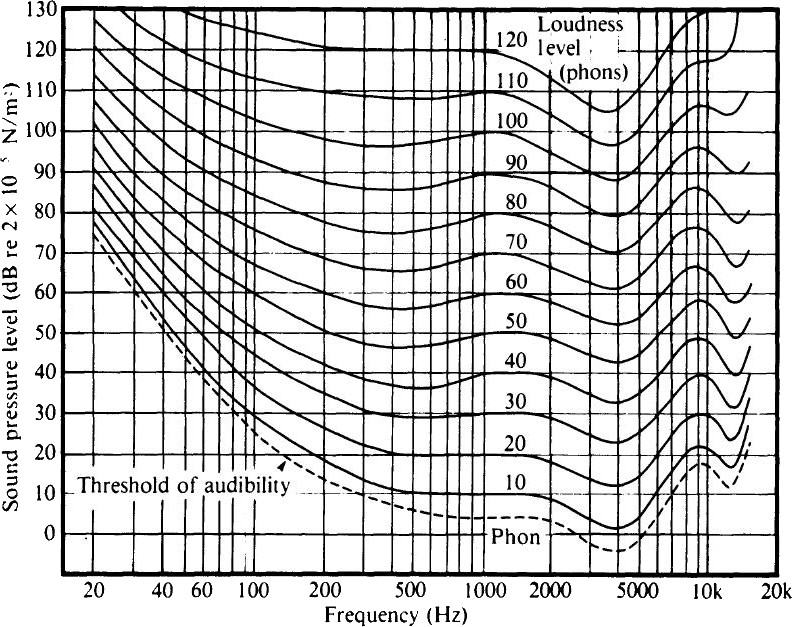
\includegraphics[width=0.6\linewidth]{00_Images/04_chapter/01.png}
    \caption{Equal-loudness contours of human hearing}
    \label{fig:equal_loudness}
\end{figure}

A second logarithmic measure concerns the energy transported by sound waves. The intensity level (IL) is defined as
\[
IL = 10 \log_{10}\left(\frac{I}{I_{0}}\right)
\]
where \( I \) is the acoustic intensity, measured in \si{\watt\per\square\metre}, and \( I_{0} = \SI{1e-12}{\watt\per\square\metre} \) is the conventional reference. For a progressive plane wave, using rms quantities, intensity can be related to acoustic pressure through
\[
I = \frac{p_{\mathrm{rms}}^2}{\rho c} = p_{\mathrm{rms}}u_{\mathrm{rms}}
\]
It is possible to observe cases where the SPL is large while the net intensity becomes negligible, for instance when energy fluxes in opposite directions balance each other (if peak amplitudes are used instead, the time-average intensity is smaller by a factor \( 1/2 \).)

\section{Normal Modes in Enclosures}

Let us consider an enclosure with a regular shape and focus on determining its normal modes. As a representative example, we take a rectangular cavity with dimensions \( a \), \( b \), and \( c \) along the three Cartesian axes. The acoustic pressure \( p(x,y,z,t) \) inside the cavity satisfies the three-dimensional wave equation
\[
\frac{\partial^{2} p}{\partial t^{2}} = c^{2}\left(\frac{\partial^{2} p}{\partial x^{2}} + \frac{\partial^{2} p}{\partial y^{2}} + \frac{\partial^{2} p}{\partial z^{2}}\right)
\]
The boundary condition at the walls can be expressed in terms of the wall acoustic impedance \( z_{w} \). Writing the pressure as \( p = z_{w} u \) and using the linear momentum equation in the frequency domain, one obtains
\[
p = z_{w} u = \frac{j z_{w}}{\rho \omega}\frac{\partial p}{\partial n}
\]
where \( \partial p / \partial n \) denotes the derivative along the outward normal to the surface. A particularly important case is that of rigid walls, for which \( z_{w} \to \infty \). In this limit the normal particle velocity vanishes, and the boundary condition becomes
\[
\frac{\partial p}{\partial n} = 0
\]
Under this assumption, a separable solution is
\[
p_{lmn}(x,y,z,t) = A \cos\left(\frac{l \pi x}{a}\right)\cos\left(\frac{m \pi y}{b}\right)\cos\left(\frac{n \pi z}{c}\right)\sin(\omega t)
\]
with \( l \), \( m \), \( n = 0,1,2,\dots \) and amplitude \( A \). The corresponding modal angular frequencies are
\[
\omega_{lmn} = \pi c\left(\frac{l^{2}}{a^{2}} + \frac{m^{2}}{b^{2}} + \frac{n^{2}}{c^{2}}\right)^{1/2}
\]
The distribution of modal frequencies depends strongly on the cavity dimension ratios. For equal ratios, multiple modes may cluster and produce pronounced coincidences, whereas more incommensurate ratios lead to a more uniform spacing, as illustrated by the mode-density plots for \( 2:2:2 \) and \( 1:2:3 \). The influence of the enclosure proportions on the modal distribution is illustrated in figure \ref{fig:mode_distribution}, comparing a cubic-like cavity with a more incommensurate set of side ratios.

\begin{figure}[!htb]
    \centering
    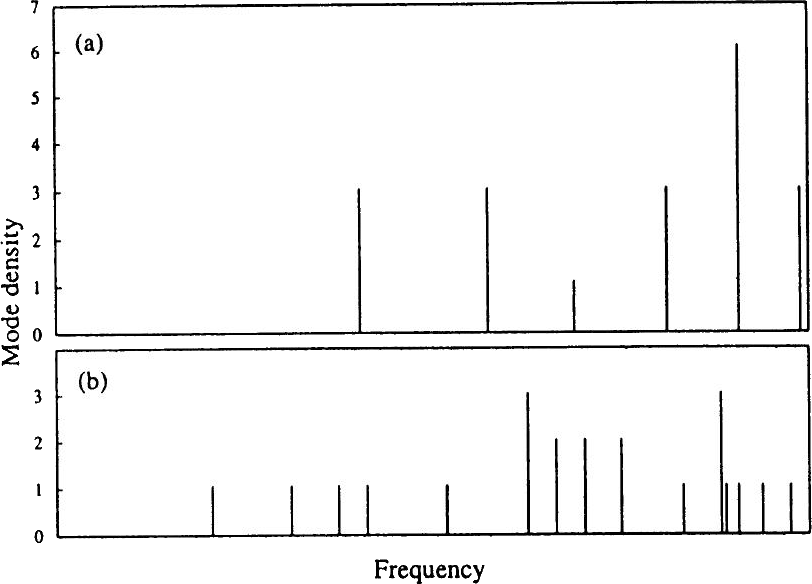
\includegraphics[width=0.6\linewidth]{00_Images/04_chapter/02.png}
    \caption{Mode distribution in a rectangular cavity for different side ratios}
    \label{fig:mode_distribution}
\end{figure}
